\documentclass[a4paper,12pt]{report}

%Русский язык
\usepackage[T2A]{fontenc}
\usepackage[utf8]{inputenc}
\usepackage[english,russian]{babel}
\usepackage{cmap}

%Работа с кодом
\usepackage{listings}
\usepackage{color}

\definecolor{green}{rgb}{0,0.6,0}
\definecolor{gray}{rgb}{0.5,0.5,0.5}
\definecolor{red}{rgb}{0.6,0,0}

\lstset{
        language=Python, 
        basicstyle=\small\ttfamily, 
        numberstyle=\tiny,           
        columns=flexible,
        stepnumber=1,                   
        numbersep=5pt,        
        showspaces=false,
        showstringspaces=false,
        showtabs=false,
        tabsize=2,                
        captionpos=b,              
        breaklines=true,           
        breakatwhitespace=false,
        keywordstyle=\color{green},
        commentstyle=\color{gray},
        stringstyle=\color{red},      
}

%Математика
\usepackage{amsmath,amsfonts,amssymb,amsthm,mathtools} 

%Изображения
\usepackage{float}
\usepackage{graphicx}
\graphicspath{ {./img/} }

%Поля страницы
\usepackage{geometry} 
\geometry{left=2.3cm} 
\geometry{right=1.8cm} 
\geometry{top=2cm} 
\geometry{bottom=2.5cm} 

%Отступы
\usepackage{indentfirst}
\setlength{\parskip}{0cm}

\begin{document} 

\begin{titlepage}
\newpage
	\begin{center}
		\large Санкт-Петербургский политехнический университет Петра Великого\\
		Институт компьютерных наук и технологий\\
		Высшая школа интеллектуальных систем и суперкомпьютерных технологий\\
	\end{center}
\vspace{7cm}

\begin{center}
		\large \textbf{Отчёт по лабораторной работе №11} \\
		\textbf{Дисциплина:} Телекоммуникационные технологии\\
		\textbf{Тема:} Модуляция и выборка (квантование)
\end{center}
\vspace{4cm}
	
\begin{flushright}
		\large Работу выполнил:\\ Ляшенко В.В.\\
		Группа: 3530901/80201\\
		Преподаватель:\\ Богач Н.В.
\end{flushright}

\vspace{\fill}
\begin{center}
	\large Санкт-Петербург\\ 2021
	\end{center}
\end{titlepage}

\tableofcontents
\listoffigures
\lstlistoflistings

\chapter{Упражнение 11.1}
    В начале мы должны для Jupyter загрузить \texttt{chap11.ipynb}, прочитать пояснения и запустить примеры.
    
    Все примеры были успешно запущены.

\chapter{Упражнение 11.2}
    В этом упражнении нам требуется посмотреть видео "D/A and A/D | Digital Show and Tell"\ Криса Монтгомери. В этом видео он демонстрирует теорему о выборках в действии и представляет множество информации о выборках. 
    
    Также в этом видео мы можем узнать, почему аналоговый звук в допустимых пределах человеческого слуха (от 20 Гц до 20 кГц) может воспроизводиться с идеальной точностью с использованием 16-битного цифрового сигнала 44,1 кГц.
    
\chapter{Упражнение 11.3}
    Вернемся к примеру "Соло на барабане"\ и применим фильтр НЧ до выборки, а затем, опять же с помощью фильтра НЧ, удалим спектральные копии, вызванные выборкой.
    
    Для начала загрузим звук барабана (Рис.3.1).
\begin{lstlisting}[caption=Получение звука барабана]
       from thinkdsp import read_wave

       wave = read_wave('263868__kevcio__amen-break-a-160-bpm.wav')
       wave.normalize()
       wave.plot()
\end{lstlisting}
\begin{figure}[H]
        \centering
        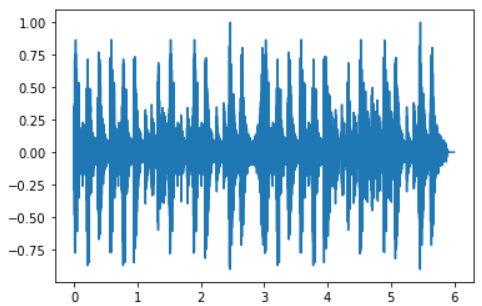
\includegraphics[width=0.8\textwidth]{fig3-1.PNG}
        \caption{Звук барабана}
        \label{fig:fig3-1}
\end{figure} 

    Данный сигнал имеет частоту дискретизации 44100 Гц.

    Теперь получим его спектр (Рис.3.2).
\begin{figure}[H]
        \centering
        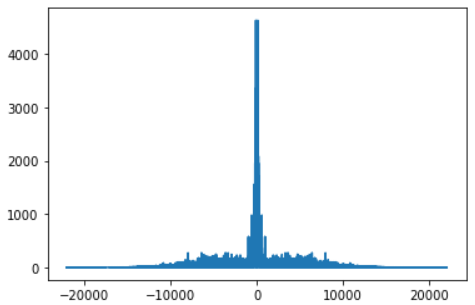
\includegraphics[width=0.8\textwidth]{fig3-2.PNG}
        \caption{Спектр сигнала}
        \label{fig:fig3-2}
\end{figure}

    Уменьшим частоту дискретизации в 4 раза. А затем перед дискретизацией мы применяем фильтр сглаживания, чтобы удалить частоты выше новой частоты свертки, которая равна частоте кадров разделённой на 2 (Рис.3.3).
\begin{lstlisting}[caption=Применение фильтра сглаживания]
       factor = 4
       framerate = wave.framerate / factor
       cutoff = framerate / 2 - 1
       spectrum.low_pass(cutoff)
       spectrum.plot()
\end{lstlisting}
\begin{figure}[H]
        \centering
        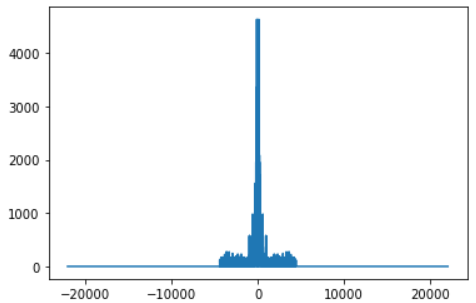
\includegraphics[width=0.8\textwidth]{fig3-3.PNG}
        \caption{Результат применения фильтра сглаживания}
        \label{fig:fig3-3}
\end{figure}
    
    Теперь воспользуемся функцией, имитирующей процесс выборки.
\begin{lstlisting}[caption=Функция выборки]
       from thinkdsp import Wave

       def sample(wave, factor):
           ys = np.zeros(len(wave))
           ys[::factor] = np.real(wave.ys[::factor])
           return Wave(ys, framerate=wave.framerate)
\end{lstlisting}     
    
    Результат применения функции содержит копии спектра, которые слегка заметны при прослушивании звука. Но их можно увидеть при построении спектра (Рис.3.4).

\begin{lstlisting}[caption=Построение спектра]
       sampled_spectrum = sampled.make_spectrum(full=True)
       sampled_spectrum.plot()
\end{lstlisting}
\begin{figure}[H]
        \centering
        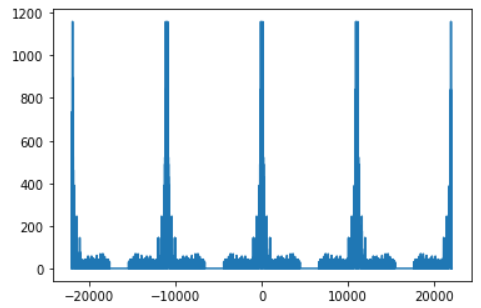
\includegraphics[width=0.8\textwidth]{fig3-4.PNG}
        \caption{Спектр после выборки}
        \label{fig:fig3-4}
\end{figure} 
    
    Мы можем избавиться от спектральных копий, снова применив фильтр сглаживания (Рис.3.5).
\begin{lstlisting}[caption=Применение фильтра сглаживания]
       sampled_spectrum.low_pass(cutoff)
       sampled_spectrum.plot()
\end{lstlisting}
\begin{figure}[H]
        \centering
        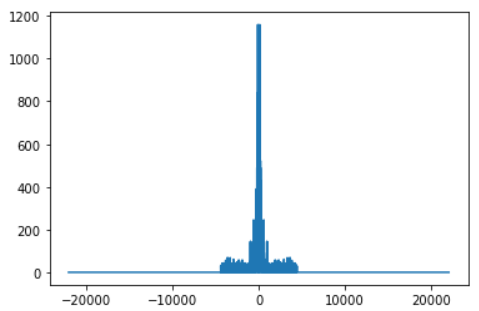
\includegraphics[width=0.8\textwidth]{fig3-5.PNG}
        \caption{Спектр после использования фильтра}
        \label{fig:fig3-5}
\end{figure}  

    Мы только что потеряли половину энергии в спектре, но мы можем масштабировать результат, чтобы вернуть её.     
\begin{lstlisting}[caption=Применение масштабирования]
       sampled_spectrum.scale(factor)
       spectrum.plot()
       sampled_spectrum.plot()
\end{lstlisting}
\begin{figure}[H]
        \centering
        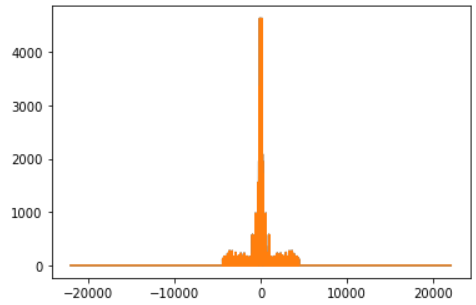
\includegraphics[width=0.8\textwidth]{fig3-6.PNG}
        \caption{Результат масштабирования}
        \label{fig:fig3-6}
\end{figure} 

    Как мы видим, между спектрами до дисктретизации и после нет большой разницы. Применение функции \texttt{max\_diff} это подтверждает. Полученная разница: $1.8749713606747085e-12$.
    
    После фильтрации и масштабирования мы можем снова получить сигнал.
\begin{lstlisting}[caption=Получение сигнала]
       interpolated = sampled_spectrum.make_wave()
       interpolated.make_audio()
\end{lstlisting}  

    Разница между интерполированным и фильтрованным сигналом также должна быть небольшой. 
\begin{lstlisting}[caption=Сравнение интерполированного и фильтрованного сигналов]
       filtered.plot()
       interpolated.plot()

       filtered.max_diff(interpolated)
\end{lstlisting}
\begin{figure}[H]
        \centering
        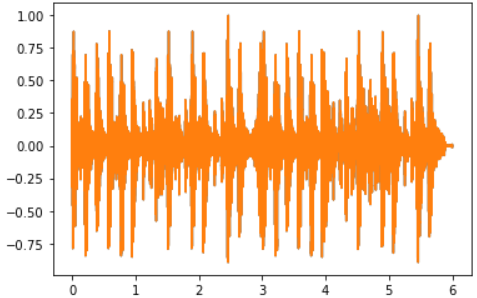
\includegraphics[width=0.8\textwidth]{fig3-7.PNG}
        \caption{Сравнение сигналов}
        \label{fig:fig3-7}
\end{figure}

    Полученная разница: $5.56290642113787e-16$.
\chapter{Выводы}
    В результате выполнения данной работы мы изучили амплитудную модуляцию, которая играет важную роль в радиосвязи, и ещё теорему о выборках, которая является важнейшей в цифровой обработке сигналов. Также мы получили навыки их применения.
\end{document}